\section{Background and Related Work}\label{sec:network:background}
This section discusses the technical background relevant to the remainder of this chapter.
First, in \refsec{sec:network:background:umts_rrc}, we introduce the \gls{UMTS} mobile communication standard, and the \gls{RRC} protocol.
Then, we discuss existing approaches to measure \gls{RRC} protocol transactions and optimise the signalling load generated by \gls{RRC} messages in \refsec{sec:network:background:measurement_optimisation}.
Finally, \refsec{sec:network:background:energy_consumption_qoe} tackles smartphone power drain and \gls{QoE}, two metrics influenced by the configuration of the \gls{RRC} protocol.

\subsection{\headershortacr{UMTS} Networks and \headershortacr{RRC} Protocol}\label{sec:network:background:umts_rrc}
A \gls{3G} \gls{UMTS} mobile network consists of three main components, which are depicted in \reffig{fig:network:background:mobile_network_overview}: the \gls{UE}, the \gls{RAN}, and the \gls{CN}.
The \gls{RAN} is used to establish connectivity between the \gls{UE} and the \gls{CN}, which in turn can establish connectivity to the Internet if required.

\begin{figure}
	\centering
	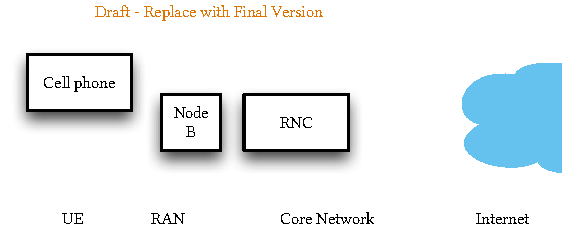
\includegraphics{network/background/figures/mobile_network_overview}
	\caption{Overview of a \gls{3G} mobile network.}
	\label{fig:network:background:mobile_network_overview}
\end{figure}

\glspl{UE} are devices used by end users, i.e. smartphones, tablets or data card enabled notebooks, but can also include \gls{M2M} devices.
The \gls{RAN} is, amongst other tasks, responsible for \gls{RRC}, packet scheduling and handover control.
It includes the NodeB and the \gls{RNC}.
The \gls{CN} provides the backbone network of the \gls{UMTS} network and provides connectivity to the Internet and the \gls{PSTN}.
Furthermore, the \gls{CN} provides billing, authentication, and location management functionalities.

\paragraph*{\headershortacr{RRC} Protocol} In \gls{UMTS} networks, the radio resources in the \gls{RAN} between base station and UE are controlled and managed by the \gls{RRC} protocol~\cite{3GPP_RRC_Spec}.
The protocol is responsible for control-band signalling between the \glspl{UE} and the \gls{RAN}.
It is used to establish, maintain, and tear down connections between a \gls{UE} and the \gls{RAN}.
Furthermore, the \gls{RRC} protocol performs broadcasting of network information, \gls{QoS} control, and reporting and cell selection management, which are out of scope for this text.
The protocol is divided into different parts: services for upper layers, communication with lower layers, protocol states, \gls{RRC} procedures, and error control.
In particular, the \gls{RRC} protocol also participates in the co-ordination of other resource management operations, channel measurements, and handovers.
All \gls{RRC} procedures rely on protocol states.
The states are defined per \gls{UE} and for the connection between the \gls{UE} and the NodeB.
Depending on the \gls{RRC} state and network activity, originating or targeted at the \gls{UE}, protocol actions can be triggered and transitions to other \gls{RRC} states may occur.
Typically there are five \gls{RRC} states characterising a connection between \gls{UE} and NodeB: \texttt{RRC\_Idle}, \texttt{URA\_PCH}, \texttt{CELL\_PCH}, \texttt{RRC\_DCH}, and \texttt{RRC\_FACH}.
Whether a specific \gls{RRC} state is used in a specific mobile network depends on the configuration of the network by the provider.
In the following we concentrate on the most commonly observed \gls{RRC} states~\cite{Qian2010a}: \gls{RRC_idle}, \gls{RRC_DCH}, and \gls{RRC_FACH}.
We omit \texttt{URA\_PCH} and \texttt{CELL\_PCH} in this study.
While \texttt{URA\_PCH} plays only a role in scenarios of high mobility, \texttt{CELL\_PCH} is not yet widely implemented.
Our results are still of general nature and do not depend on the number of considered \gls{RRC} states.

\paragraph*{\headershortacr{RRC} State Transitions} If the \gls{UE} is switched on and no data connection to the mobile network is established, the \gls{UE} is in \gls{RRC_idle} state.
If the \gls{UE} wants to send data, radio resources are allocated by the NodeB for the handset and the \gls{UE} will transition to either the \gls{RRC_FACH} or the \gls{RRC_DCH} state.
Then, a corresponding channel for data transmission is assigned to the \gls{UE} and the \gls{UE} is connected to the network.
The \gls{RRC_FACH} and the \gls{RRC_DCH} state can be distinguished in that way that in \gls{RRC_DCH} state a high-power dedicated channel for high speed transmission is allocated whereas in \gls{RRC_FACH} state a shared access channel for general sporadic data transmission is used.
Thus, \gls{RRC_FACH} consumes significantly less power than the \gls{RRC_DCH} state.

The possible transitions between the different states are defined by the network operator and the \gls{RRC} protocol stack.
Typically, the following state transitions are included:
\gls{RRC_idle} \(\rightarrow\) \gls{RRC_FACH},
\gls{RRC_FACH} \(\rightarrow\) \gls{RRC_DCH} to switch from lower radio resource utilisation and low \gls{UE} power drain to another state using more resources and power, and
\gls{RRC_DCH} \(\rightarrow\) \gls{RRC_FACH},
\gls{RRC_FACH} \(\rightarrow\) \gls{RRC_idle},
\gls{RRC_DCH} \(\rightarrow\) \gls{RRC_idle} to switch to lower resource usage and power drain.
According to~\cite{Perala2009,Qian2010a}, the transitions are triggered by user activity and radio link control buffer level at the base station.
A transition from \gls{RRC_DCH} to \gls{RRC_FACH} usually occurs when the buffer is empty and a threshold for a release timer is exceeded, resulting into the corresponding \gls{RRC} protocol message flow.
A transition in the reverse direction is triggered if the buffer level exceeds a specified threshold value for a predefined time period.
The \gls{UE} will transition into \gls{RRC_idle} state if the \gls{RNC} detects overload in the network or no data was sent by the \gls{UE} for a specified time.

\begin{figure}
	\begin{subfigure}[b]{.5\textwidth}
	\centering
	\includegraphics{network/background/figures/three_states}
	\caption{Three State Model}\label{fig:network:background:rrc_state_machines:three_states}
	\end{subfigure}
	\begin{subfigure}[b]{.5\textwidth}
	\centering
	\includegraphics{network/background/figures/two_states}
	\caption{Two State Model}\label{fig:network:background:rrc_state_machines:two_states}
	\end{subfigure}
	\caption{\headershortacr{RRC} state machine diagrams.}\label{fig:network:background:rrc_state_machines}
\end{figure}

\paragraph*{Considered Network Models} We consider two different state transition models, depicted in \reffig{fig:network:background:rrc_state_machines}, based on the \gls{RRC} protocol.
The first model including the \gls{RRC_idle}, \gls{RRC_FACH}, and \gls{RRC_DCH} states is shown in \reffig{fig:network:background:rrc_state_machines:three_states} and is in the following called the \emph{Three State Model}.
If the \gls{UE} is in the \gls{RRC_idle} state and activity is detected, i.e. a packet is sent or received, the connection transitions to \gls{RRC_DCH} state.
After each transmission a timer \TDCH is started and reset whenever a new packet is sent or received.
If the timer expires, the connection transitions to the \gls{RRC_FACH} state; upon entering, the \TFACH timer is started.
If a new transmission occurs, the connection again transitions to the \gls{RRC_DCH} state.
If \TFACH expires, the connection transitions to \gls{RRC_idle} state.

The second model, denoted as the \emph{Two State Model}, and shown in \reffig{fig:network:background:rrc_state_machines:two_states}, only includes the \gls{RRC_idle} and \gls{RRC_DCH} state.
If the \gls{UE} is in the \gls{RRC_idle} mode and a packet is sent or received, the connection transitions to the \gls{RRC_DCH} state. Once in \gls{RRC_DCH} mode, the \TDCH timer is started and it is reset whenever a new packet is sent or received.
If the timer expires, the \gls{UE} transitions back to \gls{RRC_idle} state.

\paragraph*{Proprietary Fast Dormancy Extensions} While the Three State Model is closer to the specified \gls{RRC} protocol, the Two State Model is similar to some proprietary \emph{Fast Dormancy} implementations used by \gls{UE} vendors.
In these Fast Dormancy implementations, the \gls{UE} tears down the connection to the network state as soon as no data is ready to be sent for a certain time, i.e., it forces the network to transition to \gls{RRC_idle} state.
In contrast to the Three State Model, there is no transition to the \gls{RRC_FACH} state.
If a device disconnects from the network by transitioning to the \gls{RRC_idle} state, it has to be re-authenticated before another transition to the \gls{RRC_DCH} state can occur.
This results in additional signalling traffic and causes more load on the network \cite{NSN2011} due to frequent re-establishments of the RRC connection.
These proprietary Fast Dormancy algorithms do not adhere to the \gls{RRC} specification \cite{GSM2010}, but nonetheless exist in the real world and have been identified as possible causes for signalling storms.
The major reason for Fast Dormancy implementations is the decrease in power drain on the \gls{UE}, since the transmission unit of the \gls{UE} consumes only \SIrange{1}{2}{\percent} of the power in \gls{RRC_idle} state compared to the \gls{RRC_DCH} state.
Thus, both models warrant further investigation.

\subsection{Measurements of \headershortacr{RRC} Parameters and Optimisation of Resource Consumption}\label{sec:network:background:measurement_optimisation}

In the literature the configuration of the inactivity timers used for the \gls{RRC} protocols have been investigated in detail.
In~\cite{Perala2009} a measurement tool for \gls{RRC} protocol states is presented.
It is used to determine \gls{RRC} state transition parameters, channel setup delays, and paging delay by measuring the one-way round trip time of data packets.
The results are validated by monitoring the power drain in different \gls{RRC} states.
One outcome is the observation that \gls{UMTS} network configurations vary significantly by network operator.
The \gls{RRC_DCH} release timer as well as the inactivity timer value triggering transition to \gls{RRC_idle} state were measured.
The values range from \SI{1.2}{\second} for the \gls{RRC_DCH} release timer to more than one minute for the \gls{RRC_idle} timer.
Similar results are presented in~\cite{Qian2010a}.
Here, the observed values vary between \SI{5}{\second} and \SI{12}{\second}.
Additionally, they also determined the exact \gls{RRC} state transitions for two networks, i.e. \gls{RRC_idle} \(\rightarrow\) \gls{RRC_FACH} \(\rightarrow\) \gls{RRC_DCH} or \gls{RRC_idle} \(\rightarrow\) \gls{RRC_DCH} directly without transitioning through the \gls{RRC_FACH} state.
The \gls{3GPP} has released a technical report \cite{3GPP_22801} about the adverse impact of mobile data applications.
This report states that frequent connection re-establishments due to small data packets caused by e.g. status updates of social network or instant messaging applications can lead to problems of increased signalling.
This highlights the importance of this topic.

Furthermore, there are papers that propose optimising strategies that take the \gls{RRC} states into account.
In~\cite{Qian2011a} the impact of different application traffic patterns is studied to reveal resource usage in mobile networks.
By identifying packet bursts, they infer the \gls{RRC} states of the \gls{UE}.
Radio resources are quantified by channel occupation time and power drain.
They propose an algorithm that tries to optimise application traffic patterns by e.g. piggybacking, batching up data, or decreasing the update rate of an application.
The algorithm is evaluated for six applications: two news applications, the Pandora streaming application, Google search, a Tune-In radio and Mobelix.
In~\cite{Qian2010b} \gls{RRC} states are studied for network optimisation.
The authors optimise the inactivity timers to allow a better resource utilisation.
They propose an application-to-network interface to avoid unnecessary timer periods after data transmission.

\subsection{Smartphone Power Consumption and \headershortacr{QoE}}\label{sec:network:background:energy_consumption_qoe}
As discussed at the beginning of this chapter, power drain of the \gls{UE} and the \gls{QoE} for the end user are important \glspl{KPI} for the hardware vendor and the application developer, respectively.
Power drain of the \gls{UE} varies according to the devices' current \gls{RRC} state.
The power drain caused by \gls{RRC_DCH} mode was measured on specific devices at about \SIrange{600}{800}{\milli\watt}~\cite{Qian2011a,Qian2010a}.
In \gls{RRC_FACH} mode, the power drain of an \emph{HTC TyTN II} was measured at about \SIrange{400}{460}{\milli\watt} depending on the \gls{UE} and the network operator~\cite{Qian2010a}.
A precise measurement of the power drain of different \gls{RRC} states is performed in~\cite{Qian2010a,Balasubramanian2009,Lee2004}.
The authors report that the power drain depends on two factors:
\begin{enumerate*}
\item user interactions and applications,
\item platform hardware and software.
\end{enumerate*}
Methods for reducing power drain in \gls{LTE} Machine to Machine scenarios are considered in \cite{Tirronen2012}.
The authors consider tradeoffs between responsiveness and power drain by means of prolonging the discontinuous reception cycles in the \gls{LTE} standard.
The authors of~\cite{Siekkinen2013} perform a measurement of power drain and \gls{RAN} signalling during playback of a YouTube video in \gls{3G} and \gls{LTE} \glspl{UE}.
They employ a proxy server in order to ensure that traffic is sent in bursts, thus decreasing power drain at the cost of additional signalling traffic.

In \cite{Ickin2012} the authors performed a four week long study with 29 participants to identify factors influencing the \gls{QoE} of mobile applications.
The study comprises
\begin{enumerate*}
\item data from context sensing software,
\item user feedback using an experience sampling method several times per day, and
\item weekly interviews of the participants.
\end{enumerate*}
To determine the factors of influence, the authors analyse the frequency of specific keywords in the interviews and the surveys.
They find that the term \emph{battery} is mentioned by the participants with the highest frequency.
According to the authors this is reasonable since the battery efficiency has a strong impact on the user perceived quality, in particular when the \gls{UE} is nearly discharged.
